\section{Problem}

Environments such as pipes and caves are difficult to robotically map because they are opaque and confined.  An environment is opaque when external range and vision sensors are inoperable because of lighting conditions, environmental fluids, or tight proximity to obstacles.  An environment is confined when a robot’s mobility is restricted by the close proximity to multiple obstacles.

A solution to this problem would allow mapping and exploration of previously inaccessible environments.  An approach that is invariant to ambient fluid (air, water, muddy water) would significantly impact cave exploration and underground science by the access to still deeper and smaller cave arteries regardless of whether they are submerged in water.  Search and rescue operations would have additional tools for locating survivors in complicated debris piles or collapsed mines.  Utility service workers would be able to map and inspect pipe networks without having to excavate or interrupt services.

These environments often render range sensors ineffective due to occlusions, distortions, reflections, and time-of-flight issues.  Changing visibility and lighting conditions will impact the usefulness of vision sensors.  Hazardous environments may also damage fragile external touch sensors.  This forces us to rely on a strictly proprioceptive approach for building environmental information.  Such sensors include accelerometers and joint sensors.  This sensor information is by definition, highly local to the robot’s position and sets us at a disadvantage to other mapping approaches that traditionally build maps with large sweeps of range data.  We have fundamentally less information with which to build maps and make exploration decisions.

An unstructured and irregular environment will require an agile robot with an equally agile locomotion approach.  For instance, a wheeled robot may not be capable of traversing through a complicated cave artery or debris pile but a snake robot will be able to.  Also, the geometry of the robot should not limit its ability to navigate.  For instance, a spherical robot may be able to go through a pipe of sufficient diameter, but if there is a brief pinch in the passage, the robot will not be able to continue.  The robot should be able to reposition itself to fit within the contours of the environment.

Global positioning information is also unavailable because of the enclosed nature of the environment.  Therefore, any mapping method will need an accurate motion estimation approach for the robot.  Wheeled dead-reckoning may be very difficult or impossible if the environment is highly unstructured or otherwise untenable to a wheeled locomotion approach.  Another method must be found.

\section{Related Work}

The mapping of confined spaces is a recurring theme in the research literature.  Work has been done to navigate and map underground abandoned mines [Thrun04] with large wheeled robots traveling through the constructed corridors.  Although the environment is large enough to make use of vision and range sensors, its location underground makes the use of GPS technologies problematic.  

Robotic pipe inspection has been studied for a long time [Fukuda89], but usually requires that the pipe be evacuated. The robotic solutions are often tailored for a specific pipe size and pipe structure with accompanying sensors that are selected for the task.  Often the solutions are manually remote-controlled with a light and camera for navigation.

Other work has focused on the exploration of flooded subterranean environments such as sinkholes [Gary08] and beneath sea-ice or glaciers.  This involves the use of a submersible robot and underwater sonar for sensing.

Other work has approach the problem of identifying features in the absence of external sensors.  This work comes from the robotic grasping literature and is described as “contact detection”.  That is, the identification and reconstruction of object contacts from the joint sensors of the grasping end effector.  These include Kaneko, Grupen, Haidacher, Mimura.

Finally, in addition to our early 2009 paper on this concept [Everist09], another researcher tackled the problem of mapping a confined and opaque environment of a pipe junction in an oil well bore hole deep underground [Mazzini11].  Mazzini’s approach focuses on mapping one local area of the underground oil well and uses physical probing to reconstruct the local features while anchored to a single reference frame.  
 
\section{Approach}

In this thesis, we use a snake robot in a physics simulation environment to develop a theoretical framework to map confined spaces with no external sensors.  With our simulation running the Bullet physics engine, we create a number of flat pipe-like environments in which our robot will explore and map.

We choose a snake robot form as our mapping robot due to its flexibility in moving through tight spaces and the large number of joint sensors from which we can extract environmental information. By pushing against the walls on either side of the pipe to form anchors and pulling the body forward, we achieve snake locomotion with a variation on the biological snake concertina gait.

Though we do not simulate any sensor-inhibiting fluid in the environment or sensor-failure scenarios, we prohibit ourselves from using any type of external sensor, be it touch sensors, vision sensors, or range sensors such laser range-finders and sonar.  Additionally, we do not allow ourselves to use any type of global positioning system since it is not practical to expect GPS to function underground.  The only sensors we permit ourselves to use are joint sensors.

To build the features of the environment, our robot sweeps its body through the environment and captures the free space through its body posture.   The free space becomes our dominant feature in map-making.   We use the pose graph representation for map-making, where at each pose, we build a local free space map.  We choose the geometric constraints between poses to ensure the correctness of the map.

We present several example environments, and we demonstrate the robot’s mapping and navigation results using our framework.   Our metric for success for determining the quality of a map is measured by selecting a random location on the map and judging how well the robot reliably navigates to that location in the world.

\subsection{Experimental System}

We explicitly chose to develop our approach in a simulation environment in order to rapidly develop a theoretical framework to the problem of mapping without external sensing.  In future work, we will apply these techniques to physical robots.

We choose to use the Bullet physics engine (version 2.77) because it is free, open source, mature, and actively developed.  Though it is primarily designed for games and animation, it is acceptable to our robotics application.  Our primary requisites are simulation stability and accurate modeling of friction and contact forces.   True friction and contact modeling are not available to us without specially designed simulation software at a monetary and performance speed cost.  Our choice of Bullet gives us believable results so long as we do not demand too much and try to simulate challenging situations (e.g. high speed, high mass, 1000s of contact points).

\begin{figure}
\begin{center}
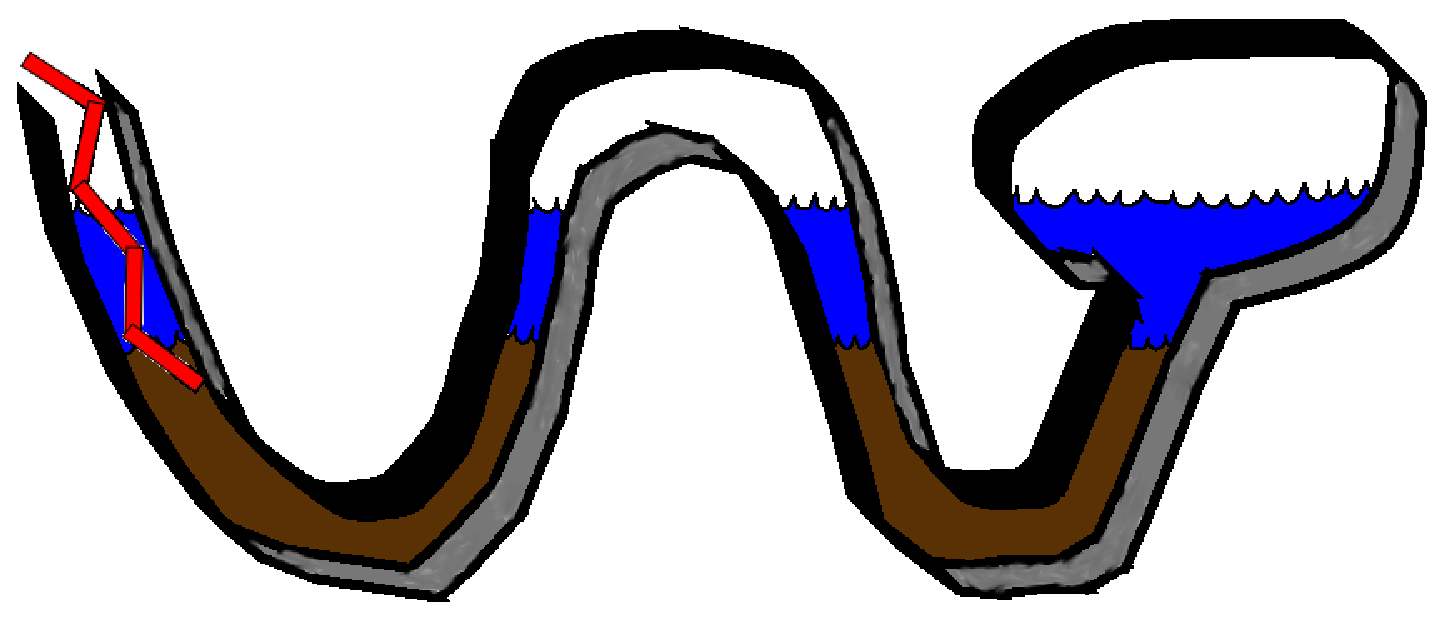
\includegraphics[scale=0.5]{rectv2-red.eps}
\end{center}
\caption{Example environment.}
\label{env1}
\end{figure}

We focus our attention on environments such as the one depicted in Figure \ref{env1}.  We build a flat plane and place a number of vertical walls to create a pipe-like maze environment.  All environments we study are flat and have no vertical components.  This means we need only focus on building 2D maps to represent the environment.  From here on in this paper, we refer to such environments as pipes even though they may not correspond to the even and regular structures of physical utility pipes.

A snake robot is placed in the pipe environment as shown in Figure \ref{env1}.  The snake robot consists of regular rectangular segments connected by actuated hinge joints.  Each of the joint axes is parallel and coming out of the ground plane.  This means the snake has no means to lift its body off the ground because all of its joints rotate in the plane of the ground.  It is only capable of pushing against the walls and sliding along the ground.  We choose a reduced capability snake robot because we wish to focus on the mapping problem instead of the more general serpentine control problem.

\begin{figure}
\begin{center}
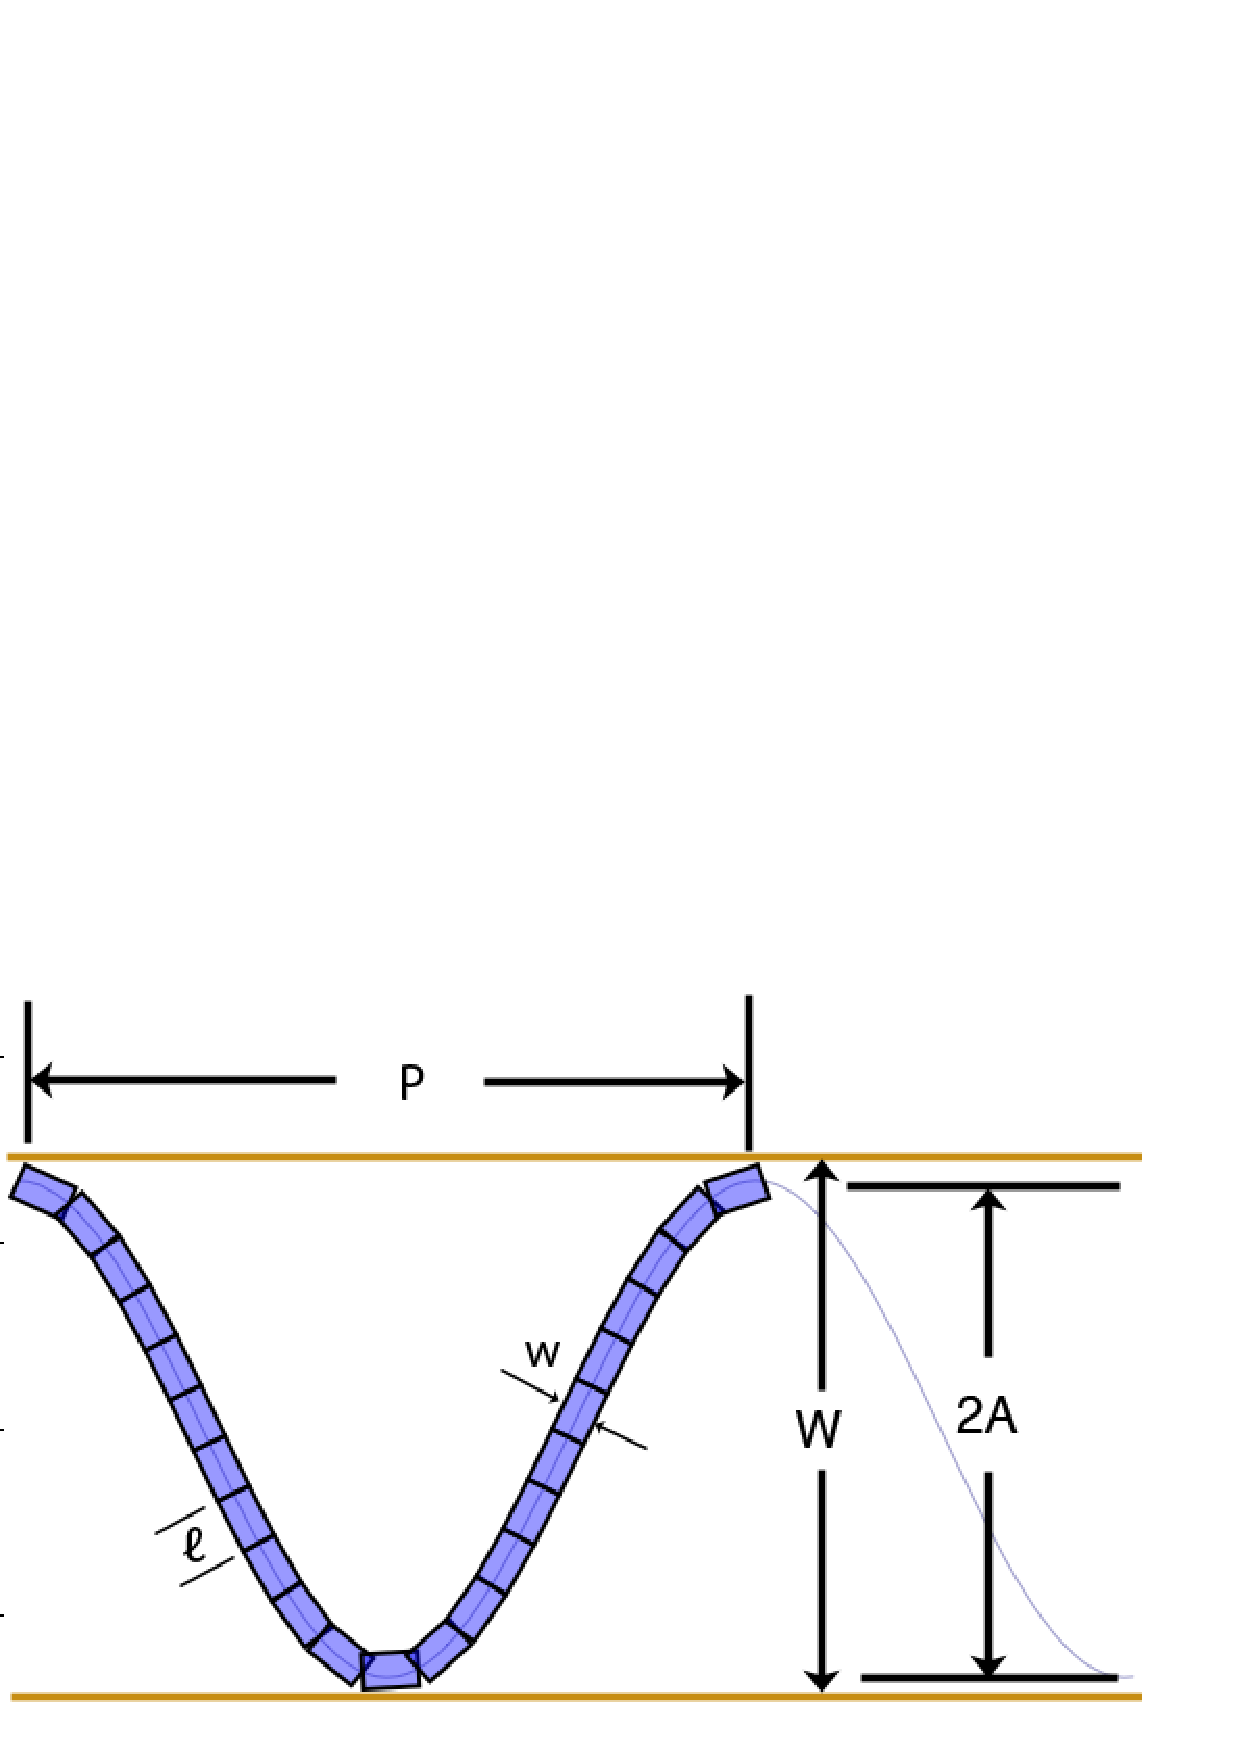
\includegraphics[scale=0.5]{CurveDiagram.png}
\end{center}
\caption{Definitions of snake and pipe parameters.}
\label{env2}
\end{figure}

We can parameterize the snake and the pipe environment.  For the snake robot, $l$ is the snake segment length, $w$ is the segment width, $N$ is the number of segments connected by $N-1$ joints, and $m$ is the maximum torque capable by each of the joint motors.

For the environment, we can begin by defining the pipe width $W$.  For a pipe with parallel and constant walls, this is a straightforward definition as seen in Figure \ref{env2}.  For non-regular features, we define the pipe width at a given point on one wall to be the distance to the closest point on the opposing wall.  This correctly captures the fact that a robot that is wider than the smallest pipe width $W$ will be unable to travel through that smallest width and will create a non-traversable pinch point.  Conversely, a pipe width $W$ that is larger than the reach of a robot will become a void space that the robot will have difficulty completely sensing without the aid of external sensors.  For both the minimum and maximum pipe widths of a given environment, we define $W_{min}$ and $W_{max}$ respectively where $W_{min} \leq W_i \leq W_{max}$ where $W_i$ is the pipe width at some point on wall $p_i$ of the pipe environment.

Each joint on the robot is actuated by a motor and PID controller.  It can actuate the joint anywhere from $\pm160$ degrees.   It uses the built-in motor capabilities of Bullet that allows us to set the joint angular velocity at run-time.  Therefore, all outputs of the PID controller set velocity commands to the joint and the physics engine does its best to satisfy those as velocity constraints.  


\begin{algorithm}
\caption{PID Controller}          % give the algorithm a caption
\label{alg1}
\begin{algorithmic}

\State $\epsilon \Leftarrow (\alpha - \phi)$

\If{$| \epsilon | > \mathrm{tol} $}

  \State $\epsilon_{sum} \Leftarrow \epsilon_{sum} + \delta t \times \epsilon$
  \State $\delta \epsilon \Leftarrow \epsilon-\epsilon_{last}$
  \State $\epsilon_{last} \Leftarrow \epsilon$
  \State $\hat{v} \Leftarrow \mathrm{P} \times \epsilon +\mathrm{I} \times \epsilon_{sum}+\mathrm{D} \times \delta \epsilon/\delta t$ 

  \If{$\hat{v} > v_{max}$}
    \State $\hat{v} \Leftarrow v_{max}$
  \EndIf
  \If{$\hat{v} < -v_{max}$}
    \State $\hat{v} \Leftarrow -v_{max}$
  \EndIf


\EndIf

\end{algorithmic}
\end{algorithm}

The structure of the PID controller is shown in Algorithm \ref{alg1}.  Line 1 defines the error as the difference between the target and the actual joint angle.  Line 2 prevents the controller from executing if the error falls below an acceptable threshold.  This prevents the motor from attempting to perform minor corrections to an already near-correct angle in order to avert oscillations or error-producing compensations.   Line 3 is the summation term for error over time while line 4 and 5 is the instantaneous error change from the previous controller iteration.  The actual PID control law is shown on line 6 where P is the proportional term coefficient, I is the integration term coefficient, and D is the derivative term coefficient.  The result outputs a command velocity for the Bullet engine.  Finally, lines 7-10 limit this velocity to a maximum.

Each of the joints gives angle position information to simulate a shaft encoder or potentiometer.  For this study, we do not simulate calibration error, sensor noise, resolution error, or gear backlash.  Calibration error has been studied elsewhere /cite and there exists correction mechanisms for it.  In the case of sensor noise, the noise on potentiometers is small enough not to affect our algorithms.  Gear backlash was encountered and studied in /cite Mazzini.  The primary error of concern is resolution error caused by the discretization process of a shaft encoder or an A/D converter.   This problem has been studied /cite.  Given a sensitive enough A/D converter (really?), this problem can be eliminated.  In this study, we assume correct and noise-free joint sensors.

A joint provides an API to the controlling program with 2 read-write parameters and 1 read-only parameter.  The read-write parameters are the target joint angle $\alpha_i$ and the maximum torque $m_i$, with the actual angle $\phi_i$ being the read-only parameter.  $\alpha_i$ is the angle in radians that we desire the joint to rotate to.  $\phi_i$ is the actual angle of the joint that reflects the current physical configuration of the robot.  $m_i$ is the maximum permitted torque that we wish to limit the individual motors to.  The maximum torque can be lowered to make the joints more compliant to the environment.



\section{Contributions}

Our contributions in this dissertation are the following:

\begin{itemize}
\item Snake movement without external sensors (Closed-loop control)
\item Proprioceptive odometer
\item Sensing with only proprioception
\item Build map with poses of local profiles that are not remotely sensible
\item Junction detection and loop-closing
\item Navigation and exploration with a proprioceptive map
\item Able to map and navigate several types of environments:  Y-junction, T-junction, X-junction, L-junction, etc.
\end{itemize}

We present our contributions in each of the subsequent chapters.

